\documentclass[a4paper,11pt]{article}
\usepackage{tabularx}
\usepackage{graphicx}
\usepackage{wrapfig}
\usepackage{subfigure}
\usepackage{enumerate}
\usepackage{natbib}
\usepackage[center,small]{caption}
\usepackage[top=2cm, bottom=2cm, left=2.5cm, right=2.5cm]{geometry} 

\title{\huge \textbf{Tutorial on using the \textit{spartan} package to analyse agent-based simulation results}\\
\Large For use with \textit{spartan} package version 1.2 onwards
\author{\Large Technique 2: One-A-Time Parameter Analysis using SpartanV Interface}
\date{}
}
\begin{document}

\maketitle


\section{Introduction}
\noindent \textit{spartan}, or (\textbf{S}imulation \textbf{P}arameter \textbf{A}nalysis \textbf{R} \textbf{T}oolkit \textbf{A}pplicatio\textbf{N}) is an R package which aids the understanding of the effect aleatory and epistemic uncertainty have on the output from a simulation. This set of tutorials makes use of available example simulation output to demonstrate how a variety of methods can be applied to further understand the results that have been generated.  Following through each example should make it easier to apply the tookit to results generated by any agent-based computer simulation.  This tutorial focuses on understanding how robust the behaviour of a simulator is to parameter perturbtation, and uses a java based interface to spartan (SpartanV) to perform this analysis.

\section{The \textit{spartan} Package}
\noindent Computer simulations are becoming a popular technique to use in attempts to further our understanding of complex systems. This package provides code for four techniques described in available literature which aid the analysis of simulation results, at both single and multiple timepoints in the simulation run. The first technique addresses aleatory uncertainty in the system caused through inherent stochasticity, and determines the number of replicate runs necessary to generate a representative result. The second examines how robust a simulation is to parameter perturbation, through the use of a one-at-a-time parameter analysis technique. Thirdly, a latin hypercube based sensitivity analysis technique is included which can elucidate non-linear effects between parameters and indicate implications of epistemic uncertainty with reference to the system being modelled. Finally, a further sensitivity analysis technique, the extended Fourier Amplitude Sampling Test (eFAST) has been included to partition the variance in simulation results between input parameters, to determine the parameters which have a significant effect on simulation behaviour.

\section{The Case Study}
\noindent The example simulation results have been taken from an ongoing project which seeks to understand the formation of lymphoid tissue in the small intestine. This simulation outputs cell behaviour measures at various points in the simulation and measures describing the development of the tissue, which occurs through interactions between these cells. Techniques 2-4 of this package allow us to explore how input parameter value affects the behaviour of these cells. We need Technique 1 to tell us how many simulation runs we need for each condition explored to ensure we have a robust representative result.

\section{Scope}
\noindent Do note that the idea of this tutorial is to demonstrate the application of the toolkit, and is not intended to act as a full introduction to using Sensitivity Analysis techniques in the analysis of simulation results. Where useful, links to further reading have been included.

\section{Prerequisites}
\begin{itemize}
\item The R statistical environment, version 2.13.1 or later.
\item The spartan R package, downloaded from the Comprehensive R Archive Network (CRAN) or from the project website.
\item The lhs and gplots R packages, available for download from CRAN.
\item The example simulation results, available from the project website.
\item From version 1.2 of \textit{spartan}, simulation results can be in either CSV or XML format. For earlier versions, results must be pre-processed to be in CSV format.
\item The SpartanV Java Interface for the spartan package. Please make sure you follow the installation instructions fully prior to running this tutorial.
\item The Parameter\_Details\_OAT.csv file available for download from the spartan website.
\end{itemize}

\section{Running Technique 2: One-A-Time (OAT) Parameter Analysis}
\noindent The robustness of a simulation to parameter alteration can be determined through the use of this approach. Following the method described by Read et al (2012), a set of parameters of interest are identified, and a range of potential values each parameter could lie within is assigned.  The technique examines the sensitivity to a change in one parameter. Thus, the value of each is perturbed independently, with all other parameters remaining at their calibrated value. In this implementation, each parameter of interest is considered in turn. Initially the parameter is assigned the minimum value within its allocated range. A number of simulation runs are then performed under these conditions (this number that which has become apparent through analysis of aleatory uncertainty, or use of Technique 1 within the \textit{spartan} package). The value of the parameter is then increased, and the runs repeated under this new criteria.  This is repeated until the full range has been explored. For each value that the parameter was assigned, the results of each simulation are examined and the median values of the output measures calculated. This creates a set of median output values for each parameter value. This set is then compared to a set of median output measures where the parameter was set to its calibrated value, using the Vargha-Delaney A-Test (2000). This gives an indication of how different the two sets of results are, and thus the change in simulation behaviour when the parameter is perturbed.\\
\\
The \textit{spartan} package includes methods to both create parameter value samples and to analyse the simulation results. This tutorial covers both methods.\\

\section{Parameter Sampling}
\noindent The package contains a method which can produce a set of values for each parameter of interest. Simulations should then be run on each of the generated parameter sets.  This is done as follows:\\
\begin{enumerate}
\item Open the SpartanV Java interface to the \textit{spartan} package. Choose Option 2: "Generate Parameter Samples for One-A-Time Analysis". Press Next.
\item Now we are going to declare the variables required by the package to produce the parameter value sets. Firstly, use the Directory Browser to select a folder where you wish your parameter value sets to be stored. Then, you need to enter details of each parameter for which you wish to create a range of value samples. You can do this in two ways:
\begin{itemize}
\item Press the "Add Parameter" button and add details on each parameter individually. These details will be name, baseline (calibrated) value, minimum value, maximum value, and an increment value between minimum and maximum.
\item Press the "Add Parameter Values From File" button. This is much more useful if you have a large number of parameters. In this tutorial, press this button and find the Parameter\_Details\_OAT.csv file you have downloaded from the website. Once you have selected this, the parameter details box will populate, as shown in Figure \ref{OAT_Screen1}. Then press Next.
\end{itemize}
\item Press the "Generate One-A-Time Parameter Samples" button. This will produce a CSV file for each parameter in the directory specified in the Directory Chooser (so in the example case, 6 are generated), with each having a name matching the parameter which is being perturbed. Simulations should then be run on each parameter value set in each file, and analysed using the technique in the next part of this tutorial.

\begin{figure}
\centering
    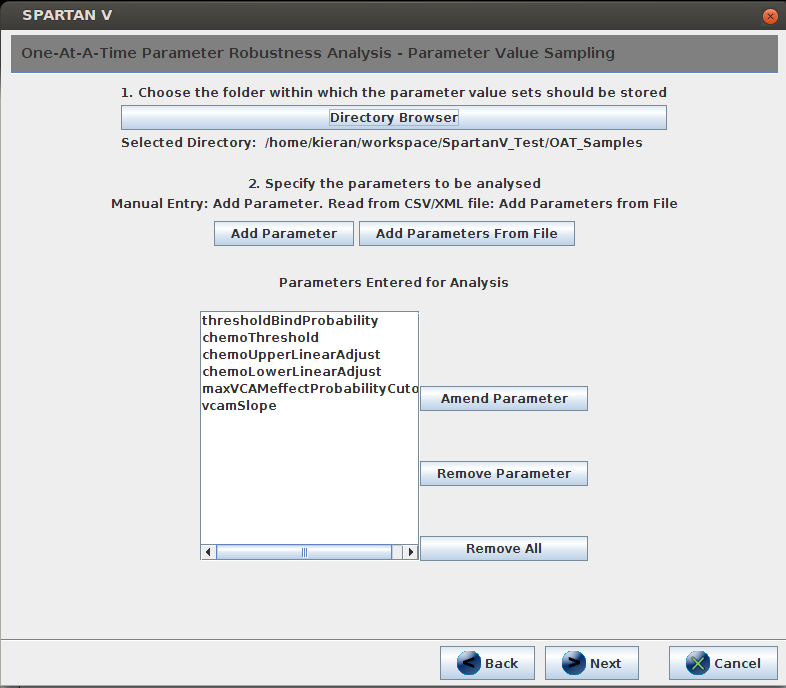
\includegraphics[width=0.8\textwidth]{SpartanV_OAT1.png}\\ \noindent
    \caption{Specifying parameter details for one-a-time parameter sampling}
    \label{OAT_Screen1}
    \newpage 
\end{figure}

\end{enumerate}

\section{Parameter Analysis}
\noindent This section of the tutorial performs this analysis for the lymphoid tissue formation simulation. In this case, we are going to examine two cell behaviour measures, Velocity and Displacement, that are captured for a period representing one hour of real time, to determine how a change in parameter value influences this behaviour. In the simulation results folders that you have downloaded from the website, the file we are going to look at is trackedCells\_Close.csv. Due to size restrictions, the example simulation results set we will analyse only examines two parameters, these being chemoLowerLinearAdjust and chemoUpperLinearAdjust. In the case study, these control expression of a chemical attractant molecule.

\begin{enumerate}
\item Download the OAT example result set from the project website and extract the results. \textbf{NB:} This is a large file, make sure it has completely downloaded else it will not extract
\item The first thing to note is the folder structure.  To use this method, the simulation results do need to be in a specific format (Figure \ref{OAT_Folders} – OAT folder structure).  The structure has three levels:
\begin{enumerate}[(i)]
\item Folders for each parameter being analysed (given that parameter name)
\item Folders for each value that the parameter has been assigned (again given that parameter value)
\item A folder for each of the simulation results where the simulation was run under those conditions. Will match the number of runs required that was determined through Aleatory Analysis (Technique 1). So, if this was 300, there would be 300 folders numbered 1-300
\end{enumerate}

\begin{figure}
\centering
    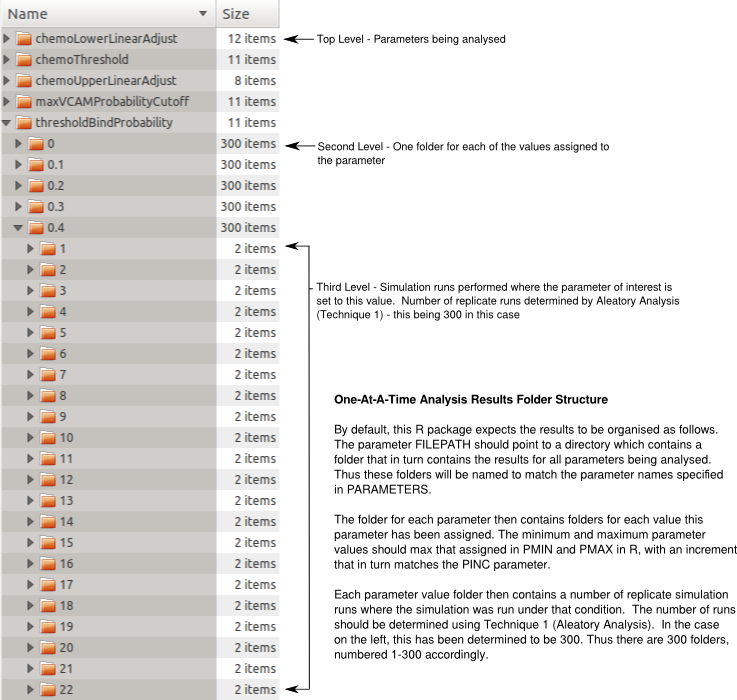
\includegraphics[width=\textwidth]{OAT_Folder_Struc.png}\\ \noindent
    \caption{Simulation results folder structure that should exist for use with this tool}
    \label{OAT_Folders}
    \newpage 
\end{figure}

\item With this data available, open the SpartanV Java interface to spartan. Select the third method from the choice of analysis methods - "Perform analysis for One-A-Time Generated Samples", and press Next.

\item You will now see the screen in Figure \ref{OAT_Screen2}. Use the Directory Browser to choose the folder that contains the results for each parameter (the folder that you have downloaded and extracted). Then you will need to enter the details of the two parameters which we are analysing. Do this by pressing the "Add Parameter" button, and enter the following data in bold:
\begin{itemize}
\item Parameter Name: \textbf{chemoLowerLinearAdjust} - Baseline: \textbf{0.04} - Minimum: \textbf{0.015} - Maximum : \textbf{0.08} - Increment: \textbf{0.005}
\item Parameter Name: \textbf{chemoUpperLinearAdjust} - Baseline: \textbf{0.2} - Minimum: \textbf{0.1} - Maximum : \textbf{0.5} - Increment: \textbf{0.05}
\end{itemize}

Your screen should look like that shown in Figure \ref{OAT_Screen2}. Press Next.

\begin{figure}
\centering
    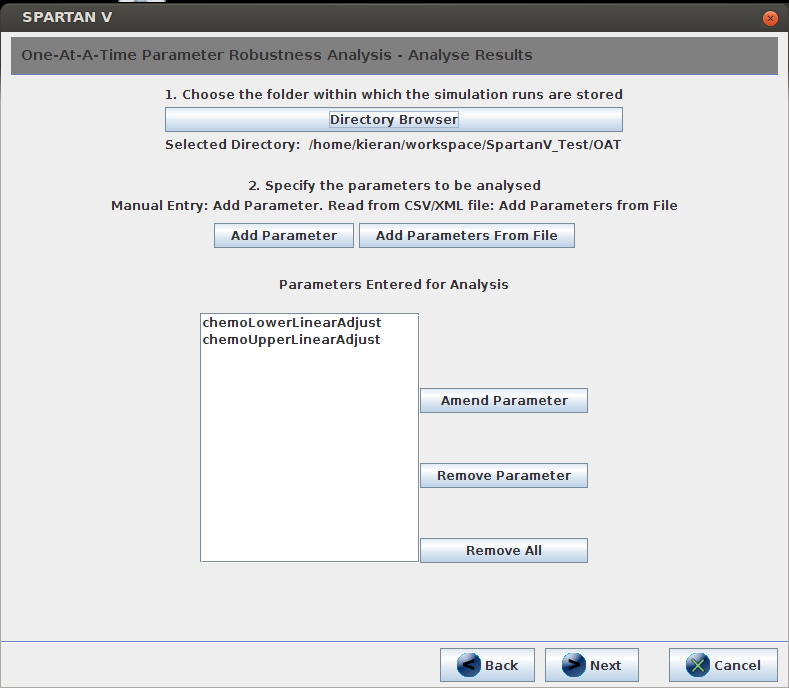
\includegraphics[width=0.8\textwidth]{SpartanV_OAT2.png}\\ \noindent
    \caption{Specifying parameter details for one-a-time analysis}
    \label{OAT_Screen2}
    \newpage 
\end{figure}

\item You will now see the screen in Figure \ref{OAT_Screen3}. This screen requests information about the simulator, in terms of output type (spartan can process XML or CSV), result file names, and particular columns where the output responses can be found (if csv). For CSV output, it is good to specify result start and end columns to save R errors on duplicate first column entries, and to save reading in whole CSV files. Finally, the screen requests information on simulation timepoints that are being examined. This is covered later in the tutorial. In this scenario, we assume we are only examining one timepoint, and this the last two input boxes are set to NULL. Complete the input boxes with the data shown in Figure \ref{OAT_Screen3} and click Next.

\begin{figure}
\centering
    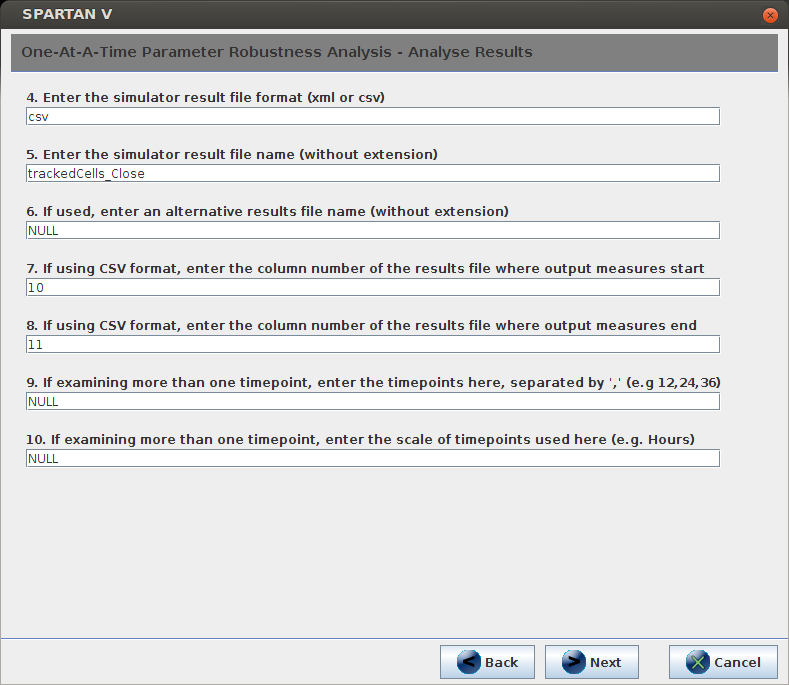
\includegraphics[width=0.8\textwidth]{SpartanV_OAT3.png}\\ \noindent
    \caption{Specifying simulation specifics for this method of analysis}
    \label{OAT_Screen3}
    \newpage 
\end{figure}

\item The next screen (as shown in Figure \ref{OAT_Screen4}) requests information on the simulation output responses that have been examined, the number of replicate runs performed for each parameter value (if this is the case, e.g. for stochastic simulations), and names to assign file names created by the analysis. The last entry is the statistical limit of the Vargha-Delaney A-Test where the difference between the behaviour that becomes apparent under a new parameter value and behaviour under normal circumstances is deemed to be 'large'. This is a default value and can be left as such. Complete the data input boxes as shown in Figure \ref{OAT_Screen4} and  press Next.

\begin{figure}
\centering
    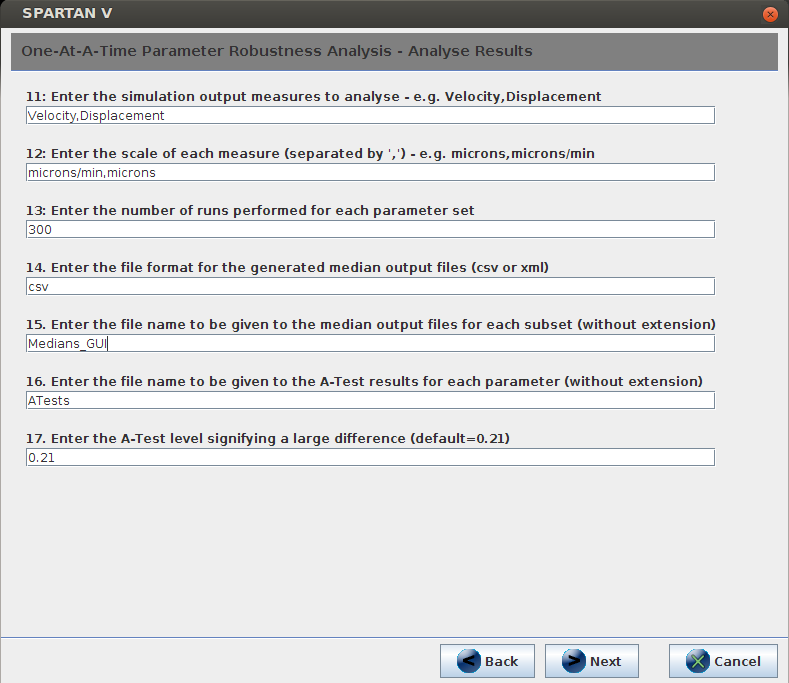
\includegraphics[width=0.8\textwidth]{SpartanV_OAT4.png}\\ \noindent
    \caption{Specifying simulation specifics for this method of analysis}
    \label{OAT_Screen4}
    \newpage 
\end{figure}

\item The final screen asks what methods you wish to run in this analysis. Although you would normally run them all, you may want to run some of these separately, or perform them at different times. In this case, we are going to run all four. These are:

\begin{verbatim}
oat_processParamSubsets(FILEPATH,PARAMETERS,PMIN,PMAX,PINC,
NUMRUNSPERSAMPLE,MEASURES,RESULTFILEFORMAT,RESULTFILENAME,
ALTERNATIVEFILENAME,OUTPUTCOLSTART,OUTPUTCOLEND,
MEDIANSFILEFORMAT,MEDIANSFILENAME)
\end{verbatim}

This examines each parameter that is to be analysed in turn, starting with the minimum value it has been assigned and works through all values up to and including the maximum in the range.  For each value, the median of each output measure is calculated for each run that has been performed, and these stored in a file within the folder for this parameter value (file given the name set in MEDIANSFILENAME entry box). For example, if the parameter value is 0, and 300 runs have been performed where this is the case, a file is created containing the median of both the Velocity and Displacement output measure for each of the 300 runs. This will be in CSV or XML format, dependent on the format set by parameter MEDIANFILEFORMAT. This set of medians can then be compared with the known simulation behaviour at the baseline.

\begin{verbatim}
oat_analyseAllParams(FILEPATH,PARAMETERS,BASELINE,PMIN,
	PMAX,PINC,MEASURES,MEDIANSFILEFORMAT,MEDIANSFILENAME,
	ATESTRESULTSFILENAME)
\end{verbatim}

Again, this method examines each parameter in turn.  The aim is to compare the median sets generated above with those obtained when the parameter was set to its calibrated, baseline, value.  As an example, consider one of the parameters we are analysing in the example set, chemoLowerLinearAdjust.  This has a baseline value of 0.04. The simulation has two output measures, Velocity and Displacement. The method will read in the median results generated by the first method where the parameter value is its calibrated value. Then, it will, in turn, read in the median results for every other parameter value. So, for example, the minium value for chemoLowerLinearAdjust is 0.015. The method will read in the medians for all simulation runs for this value. For each output measure, the sets of median values are then compared using the Vargha-Delaney A-Test (2000), which indicates 'how different' the two sets of results are, or the effect the parameter value change has had on the simulation result. The next value for this parameter is then considered, and the same process followed.  Once this is all complete, the A-Test scores for each parameter value comparison are output to a CSV file.\\

\begin{verbatim}
oat_graphATestsForSampleSize(FILEPATH,PARAMETERS,PMIN,
	PMAX,PINC,MEASURES,ATESTSIGLEVEL,
	ATESTRESULTSFILENAME,TIMEPOINTS,TIMEPOINTSCALE)

oat_plotResultDistribution(FILEPATH,PARAMETERS,PMIN,
	PMAX,PINC,MEASURES,MEASURE_SCALE,MEDIANSFILEFORMAT,
	MEDIANSFILENAME,TIMEPOINTS,TIMEPOINTSCALE)
\end{verbatim}

The first of these methods produces a graph for each parameter, which shows the A-Test scores for each value it has been assigned, when compared to its calibrated value. This plot will show all simulation output measures on the same graph. This helps identify any trends that become apparent when the value of a parameter is changed. 
\\
The final method again produces a graph for each parameter, but this time also for each simulation output measure. This generates a box plot showing the distribution of simulation results for that measure, for each parameter value, again making it easy to identify any trends in simulation behaviour against parameter value. 

\item Press Next, and then press the "Run One-A-Time Robustness Analysis" button. The analysis will now run, with updates provided in the console. When the analysis has finished, the following will be produced:
\begin{itemize}
\item A summary of A-Test scores for each value assigned to each parameter. This will be within the parameter folder, and in this case called ATests.csv
\item A graph of this data, for each parameter, again in the same folder. Two examples can be seen in Figures \ref{OAT_Results1} and \ref{OAT_Results2}. In this example a notable change in simulation behaviour is identified when the value of chemoLowerLinearAdjust is perturbed (Figure \ref{OAT_Results1}). Or on the other hand, it may become apparent that the value of the parameter can be set to any value in the range and there be no notable change in simulation behaviour. This is the case with the chemoUpperLinearAdjust parameter, in Figure \ref{OAT_Results2}.
\item A plot of the distribution of simulation responses for each parameter value. One of the graphs produced in this case can be seen in Figure \ref{OAT_Results3}.
\end{itemize}


\end{enumerate}
\newpage 
\begin{figure}[h!]
\centering
    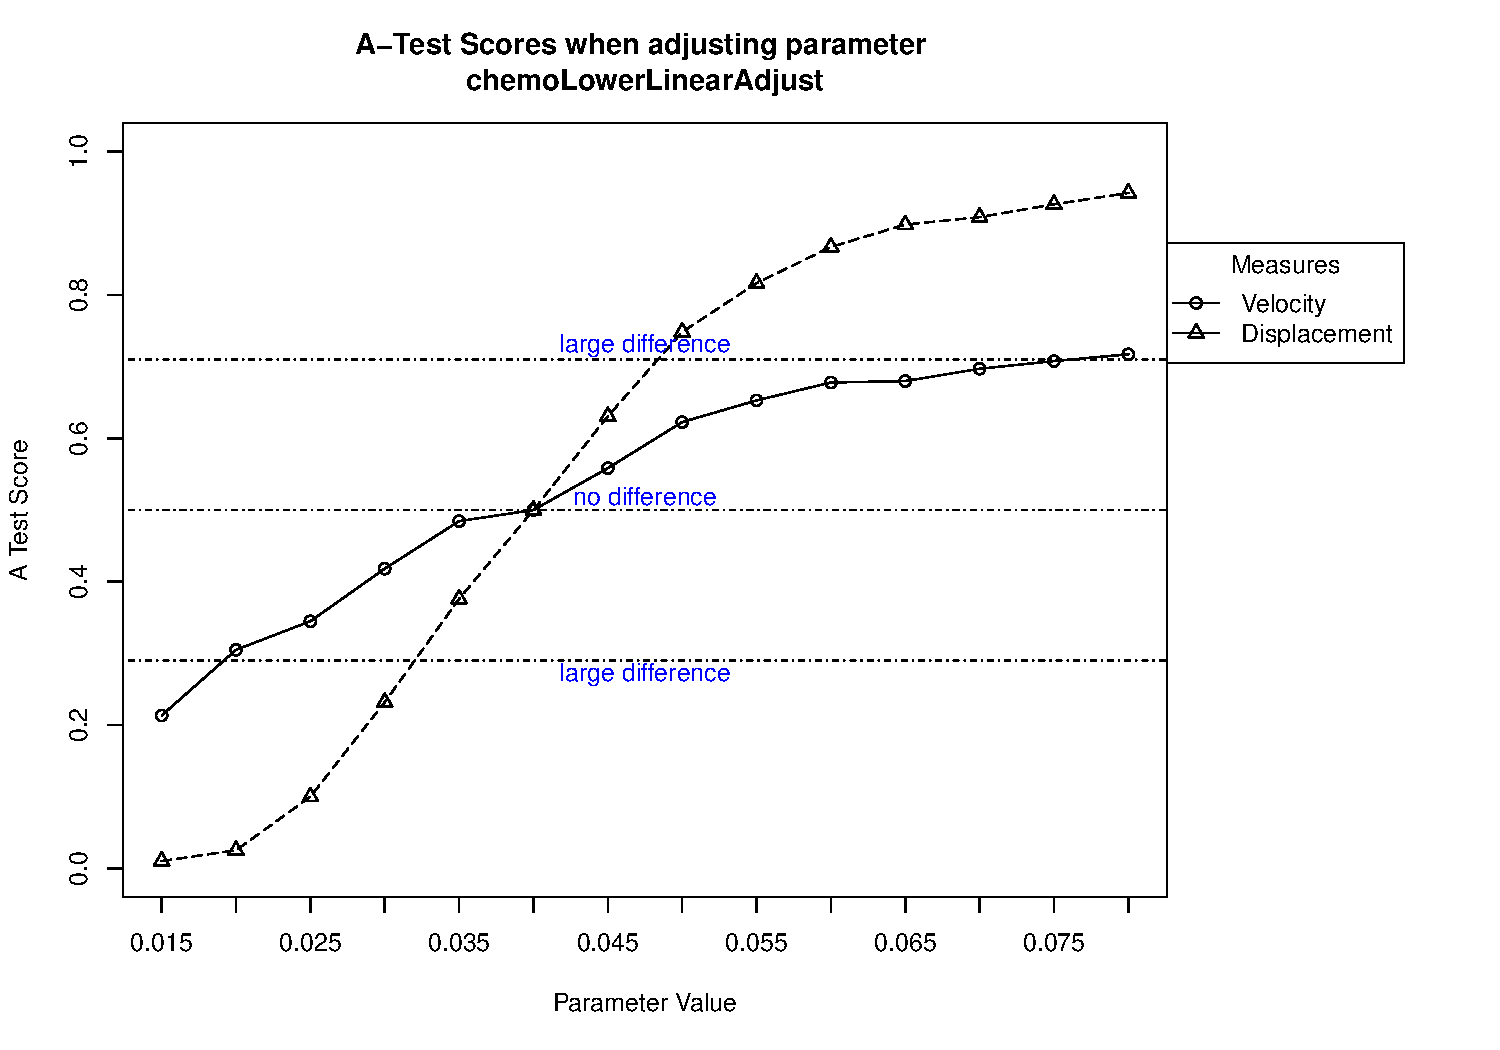
\includegraphics[width=0.9\textwidth]{OAT_chemoLowerLinearAdjust.pdf}\\ \noindent
    \caption{Graph showing the A-Test scores for all parameter values assigned to chemoLowerLinearAdjust}
    \label{OAT_Results1}
    \end{figure}

\begin{figure}[h!]
\centering
    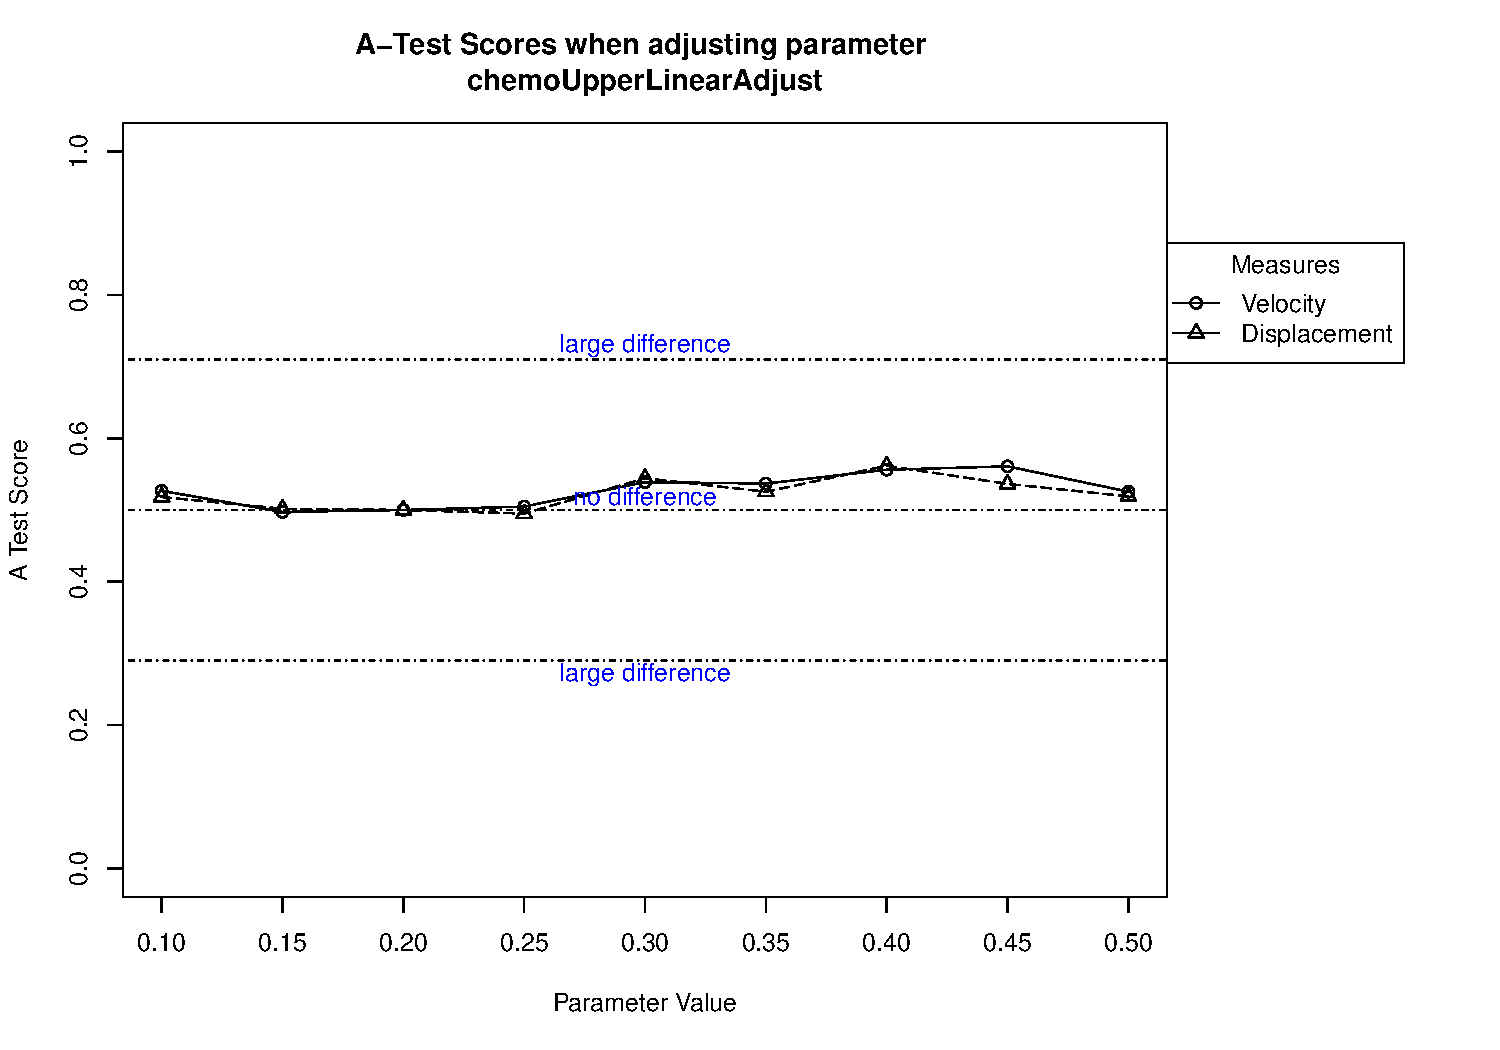
\includegraphics[width=0.9\textwidth]{OAT_chemoUpperLinearAdjust.pdf}\\ \noindent
    \caption{Graph showing the A-Test scores for all parameter values assigned to chemoUpperLinearAdjust}
    \label{OAT_Results2}
\end{figure}

\newpage 
\begin{figure}[h!]
\centering
    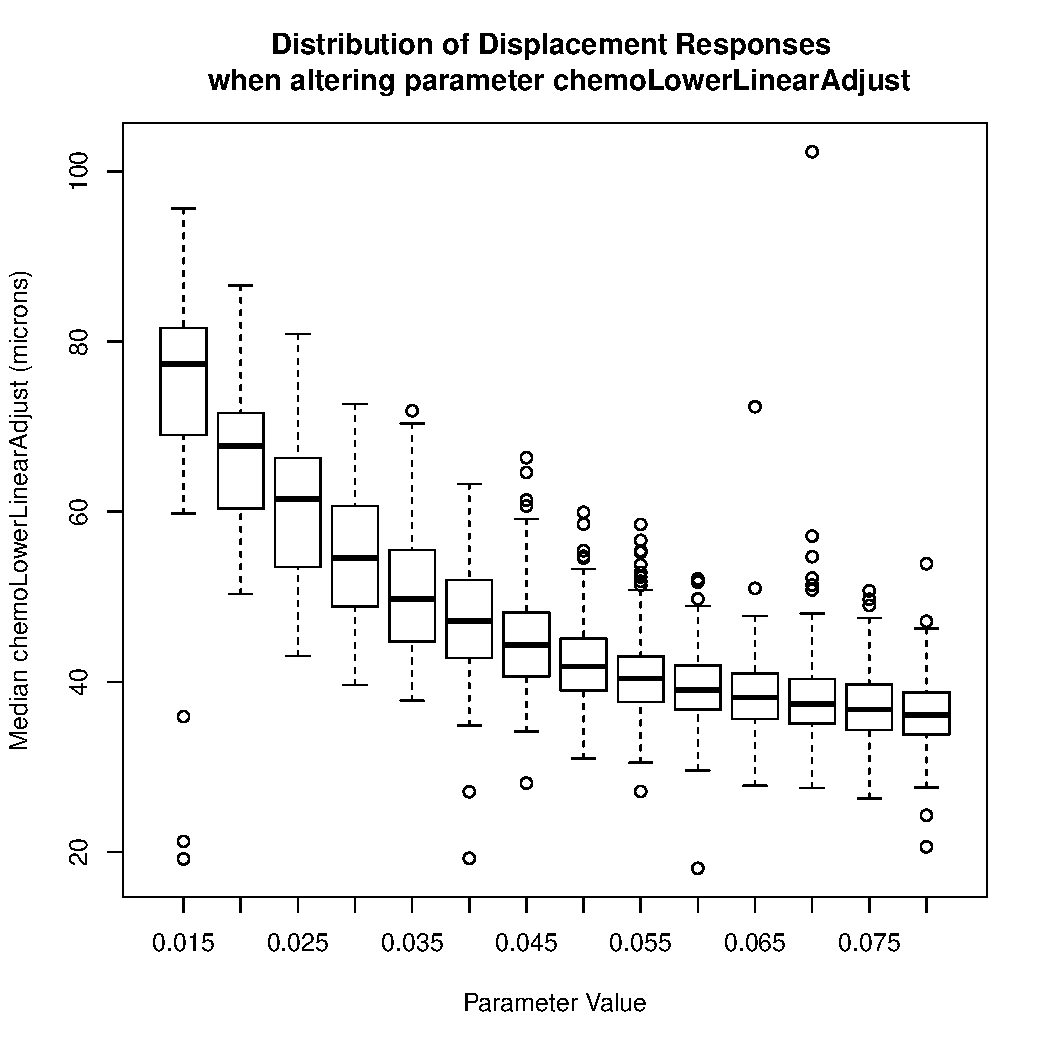
\includegraphics[width=0.9\textwidth]{chemoLowerLinearAdjust_DisplacementBP.pdf}\\ \noindent
    \caption{Graph showing the distribution of Displacement results when parameter chemoLowerLinearAdjust is perturbed}
    \label{OAT_Results3}
    \end{figure}

\section{Running OAT Technique for Multiple Timepoints}
\noindent The package also has the capability to perform the above analysis for simulation results taken at different timepoints. This may give an indication of when a parameter perturbation becomes influential.  Again, we will examine this with an example, yet there is not much to change from the example seen previously\\
\\
In this case study, we have captured the cell behaviour measures at multiple timepoints in the simulation, specifically 12, 36, 48,and 60 hours. Thus we have the output files trackedCells\_Close\_12.csv, trackedCells\_Close\_36.csv etc. To use this method over multiple timepoints, you should have (a) the same folder structure as in the previous example, and (b) an output file for each timepoint, with the timepoint appended to the filename after an underscore. It is worth writing a script to put your output in this format before looking at this method if this is not already the case.
\\
Launch the SpartanV interface, and complete Steps 1-4 in the same way as that above. Now, on the second data input screen, enter 12,36,48,60 into box 9 (Timepoints) and type Hours into box 10 (timepoint scale), as seen in Figure \ref{OAT_Screen5}. This tells the analysis that you want to examine simulation responses at four different time-points, with the latter used for graphing results in the final part of the method. Press Next and complete the other data entry screens in the same way. Run the analysis, and statistics will be produced for all four timepoints.

\begin{figure}
\centering
    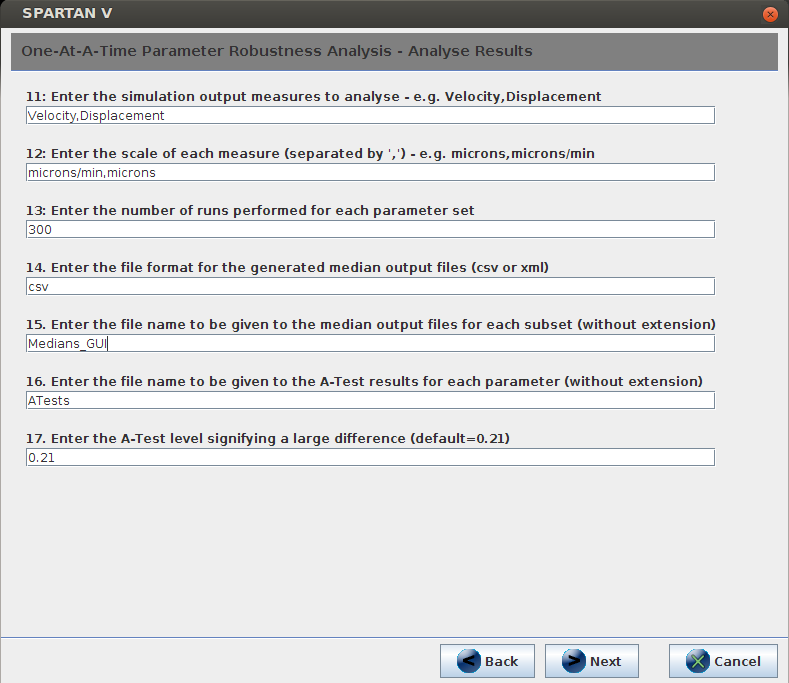
\includegraphics[width=0.8\textwidth]{SpartanV_OAT4.png}\\ \noindent
    \caption{Adding additional time-points to observe effect of parameter perturbation over time}
    \label{OAT_Screen5}
    \newpage 
\end{figure}


\section{Further Reading}
\noindent
The following references may be useful in understanding this technique in more detail:
\begin{itemize}
\item Read, M., Andrews, P.S., Timmis, J. \& Kumar, V. (2012) Techniques for Grounding Agent-Based Simulations in the Real Domain : a case study in Experimental Autoimmune Encephalomyelitis. Mathematical and Computer Modelling of Dynamical Systems, 18(1):67-86.
\item Vargha, A. \& Delaney, H.D. (2000) A critique and improvement of the CL Common Language Effect Size Statistics of McGraw and Wong. Journal of Educational and Behavioural Statistics, 25, p.pp.101-132.
\item The spartan Manual, spartan-Manual.pdf, within the spartan package describes in more detail each method within the package
\end{itemize}


\end{document}